% !TeX spellcheck = en_GB
%%%%%%%%%%%%%%%%%%%%%%%%%%%%%%%%%%%%%%%%%%%%%%%%%%%%%%%%%%%%%%%%%%%%%%%%%%%%%%%%
%\documentclass[handout]{beamer}\mode<handout>{\usetheme{default}}
%
\documentclass[presentation]{beamer}\mode<presentation>{\usetheme{blackAMSBolognaFC}}
%\documentclass[handout]{beamer}\mode<handout>{\usetheme{AMSBolognaFC}}
% \setbeamertemplate{bibliography item}{\insertbiblabel}
%%%%%%%%%%%%%%%%%%%%%%%%%%%%%%%%%%%%%%%%%%%%%%%%%%%%%%%%%%%%%%%%%%%%%%%%%%%%%%%%
\usepackage[english]{babel}
\usepackage[utf8]{inputenc}
%
\usepackage{magnini-dc-kr-2023}
%%%%%%%%%%%%%%%%%%%%%%%%%%%%%%%%%%%%%%%%%%%%%%%%%%%%%%%%%%%%%%%%%%%%%%%%%%%%%%%%
\title[Symbolic Transfer Learning]{
    % same title of the presented paper
    \textbf{Symbolic Transfer Learning through}
    \\
    \textbf{Knowledge Manipulation Methods}
}
%
% \subtitle{Extended Abstract}
%
% same authors order of the presented paper
\author[Magnini]{
	\emph{Matteo Magnini}$^{*}$ % empth the presenting author
}
%
\institute[UniBo]{
    $^{*}$Dipartimento di Informatica -- Scienza e Ingegneria (DISI)
    \\
    \textsc{Alma Mater Studiorum} -- Università di Bologna
    \\
    \texttt{
        \emph{matteo.magnini}@unibo.it % emph the presenting author's email
    }
}
%
\date[DC KR 2023]{
	Doctoral Consortium at the
    \\
    20\textsuperscript{th} International Conference on
	\\
	Principles of Knowledge Representation and Reasoning (KR)
	\\
	September 5\textsuperscript{th}, 2023, Rhodes (Greece)
}
%%%%%%%%%%%%%%%%%%%%%%%%%%%%%%%%%%%%%%%%%%%%%%%%%%%%%%%%%%%%%%%%%%%%%%%%%%%%%%%%
\AtBeginSection[]
{
%\\\\\\\\\\\\\\\\\\\\\
\begin{frame}<beamer>[c,noframenumbering]
\frametitle{Next in Line\ldots}
\tableofcontents[sectionstyle=show/shaded,subsectionstyle=hide]
\end{frame}
%\\\\\\\\\\\\\\\\\\\\\
}
\AtBeginSubsection[]
{
%\\\\\\\\\\\\\\\\\\\\\
\begin{frame}<beamer>[shrink,noframenumbering]
    \frametitle{Focus on\ldots}
	\mbox{~}
	\tableofcontents[currentsubsection,sectionstyle=shaded,subsectionstyle=show/shaded]
	\mbox{~}
\end{frame}
%\\\\\\\\\\\\\\\\\\\\\
}
%%%%%%%%%%%%%%%%%%%%%%%%%%%%%%%%%%%%%%%%%%%%%%%%%%%%%%%%%%%%%%%%%%%%%%%%%%%%%%%%
\begin{document}
%%%%%%%%%%%%%%%%%%%%%%%%%%%%%%%%%%%%%%%%%%%%%%%%%%%%%%%%%%%%%%%%%%%%%%%%%%%%%%%%

%\\\\\\\\\\\\\\\\\\\\\
\frame{\titlepage}
%\\\\\\\\\\\\\\\\\\\\\

%===============================================================================
\section{Motivation \& Context}
%===============================================================================

%\\\\\\\\\\\\\\\\\\\\\
\begin{frame}[c]{Context}

    Players involved in a Machine Learning workflow:
    \vspace{0.5cm}
    \begin{itemize}
        \item Data
        %
        \begin{itemize}
            \item[!] require \alert{labels}
        \end{itemize}

        \vfill

        \item Knowledge
        %
        \begin{itemize}
            \item human experts
            \item common sense
            \item extracted from data/models
        \end{itemize}

        \vfill

        \item Model
        %
        \begin{itemize}
            \item trained on data
            \item sometimes also trained with prior knowledge
        \end{itemize}

    \end{itemize}
\end{frame}
%\\\\\\\\\\\\\\\\\\\\\

%\\\\\\\\\\\\\\\\\\\\\
\begin{frame}[allowframebreaks]{Utopy and Reality}

    \hspace{0.5cm}
    \includegraphics[width=0.4\textwidth]{figures/data-labels-knowledge-1}
    \hfill

    \framebreak

    \hspace{0.5cm}
    {\transparent{0.2}\includegraphics[width=0.4\textwidth]{figures/data-labels-knowledge-1}}
    \hfill
    \includegraphics[width=0.4\textwidth]{figures/data-labels-knowledge-2}
    \hspace{0.5cm}

    \framebreak

    \centering
    But in some tasks we deal with both low data/labels and knowledge\dots

\end{frame}
%\\\\\\\\\\\\\\\\\\\\\

%\\\\\\\\\\\\\\\\\\\\\
\begin{frame}[allowframebreaks]{Transfer Learning}

    \centering
    Reuse the knowledge acquired in a \alert{similar} task!~\ccite{transfer-learning-survey-Tan-2018}

    \framebreak

    \begin{figure}
        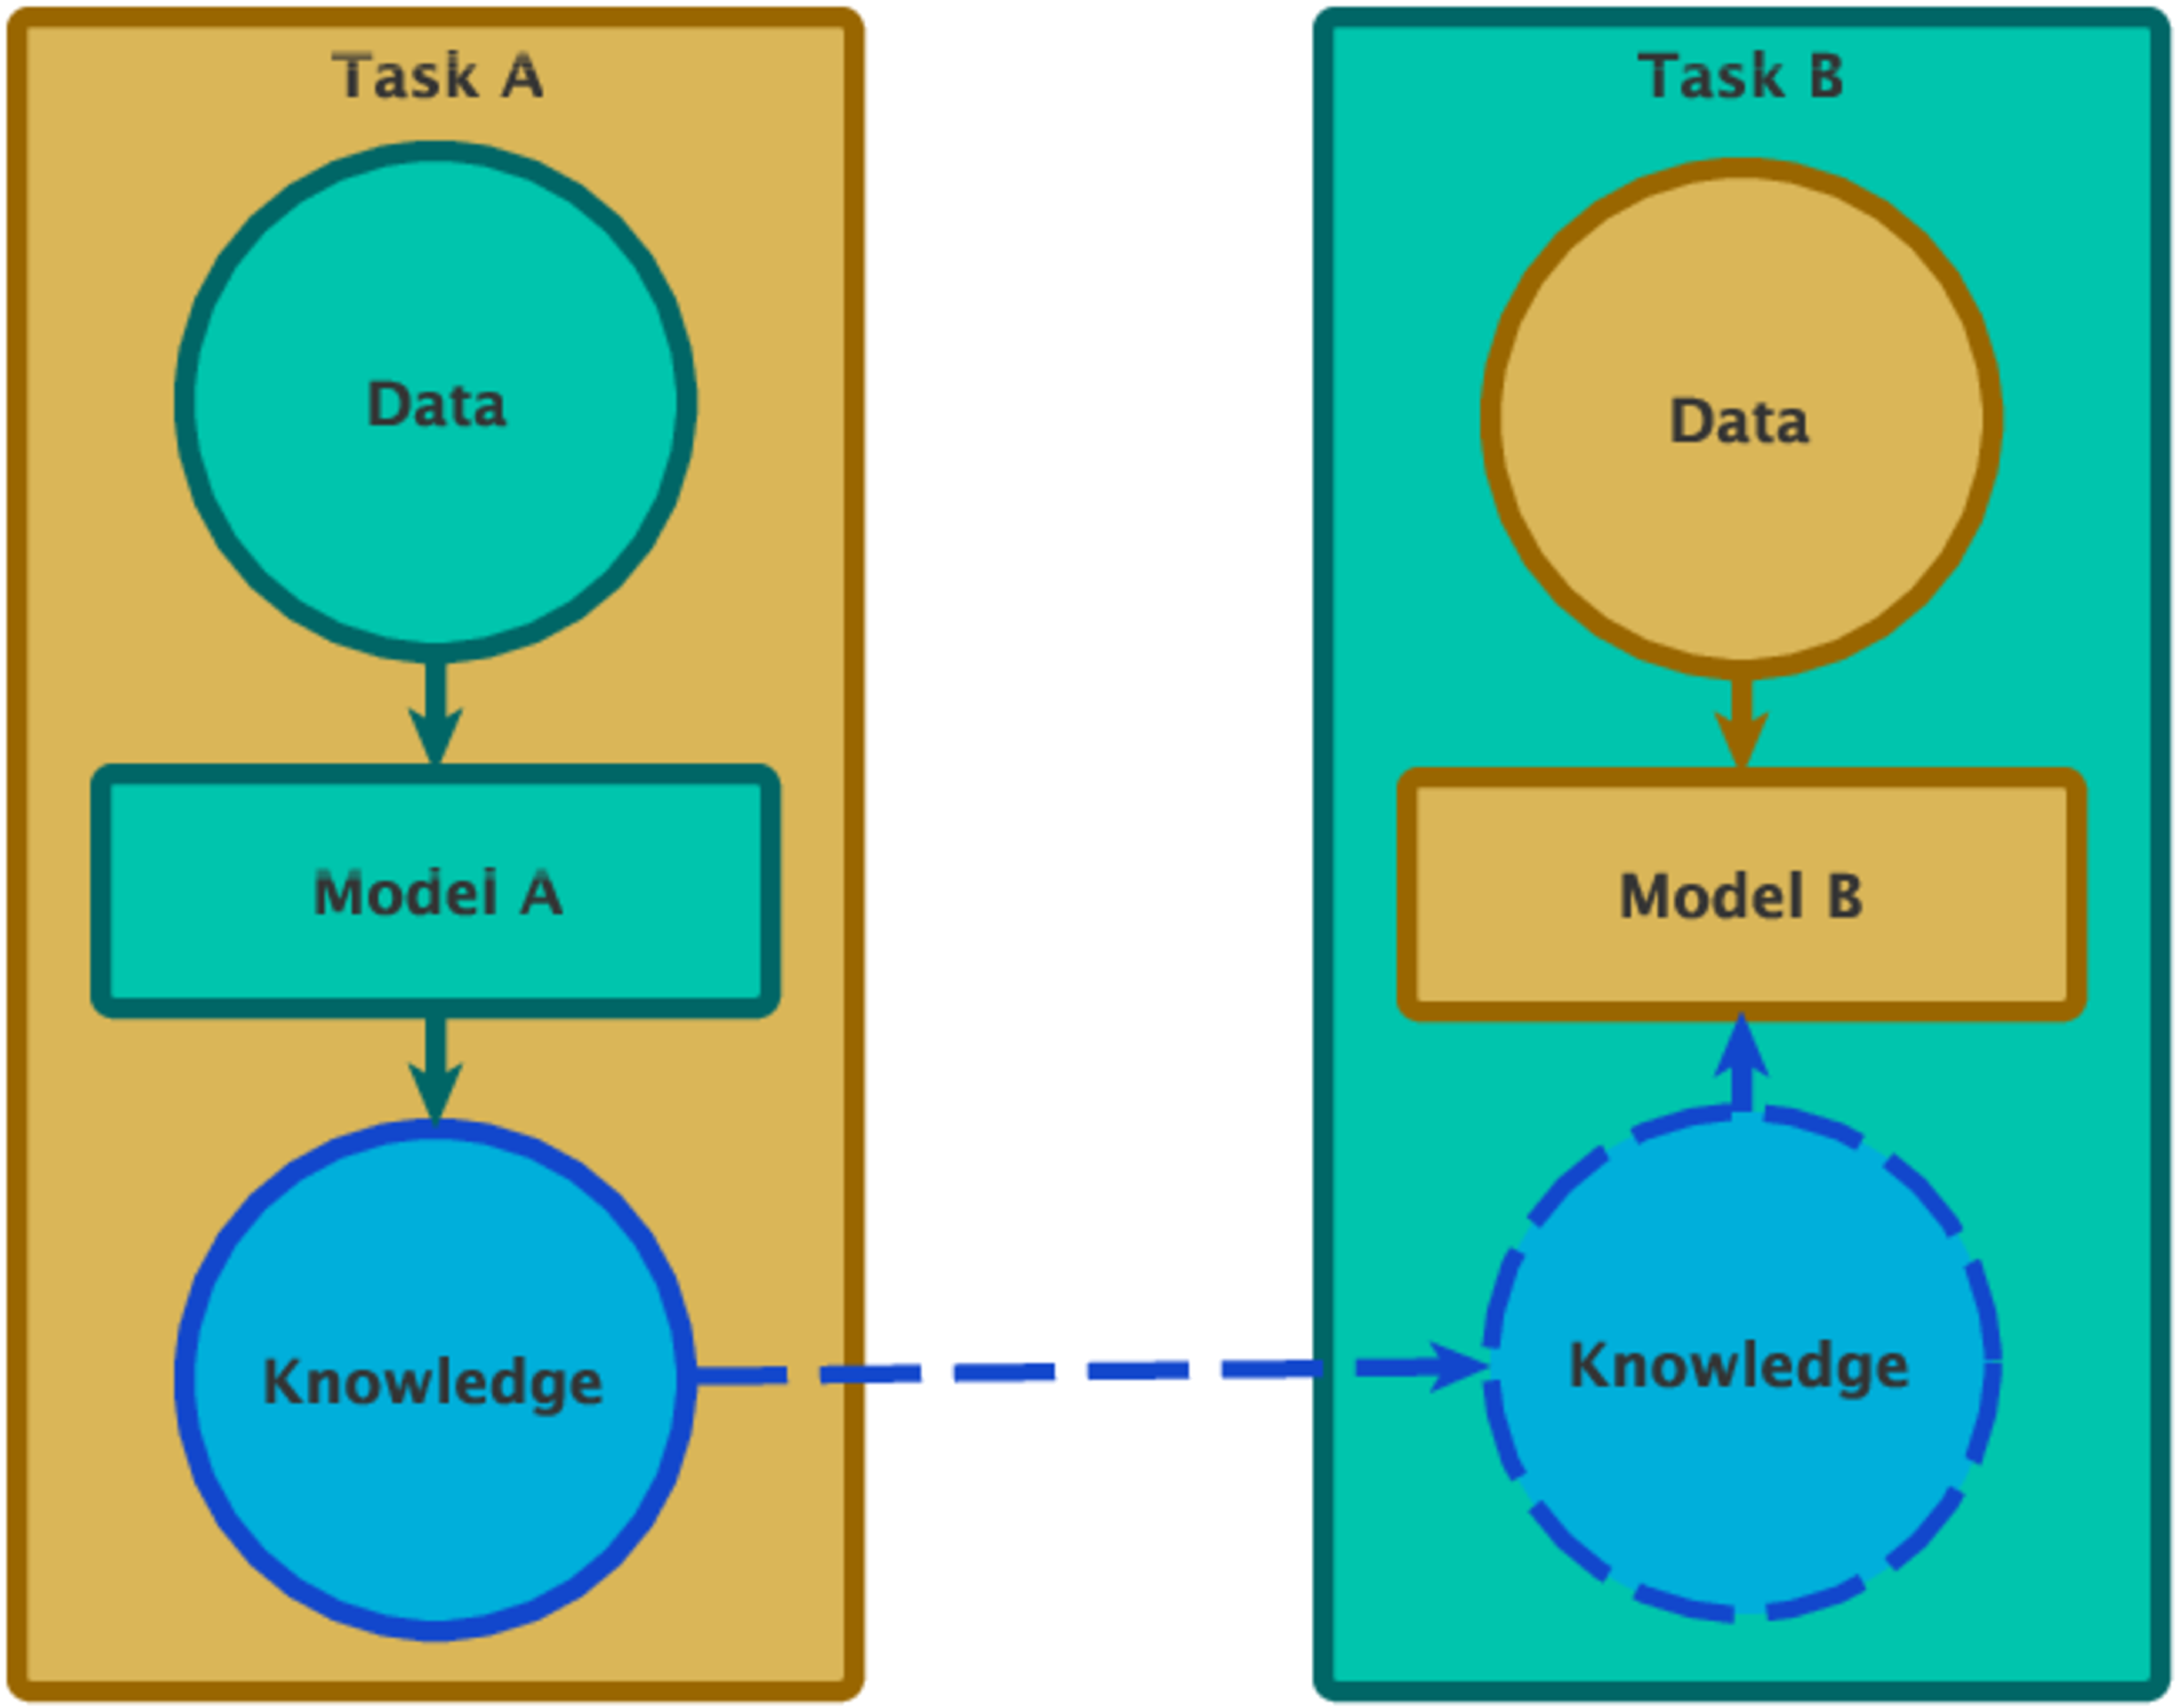
\includegraphics[width=0.7\textwidth]{figures/transfer-learning}
    \end{figure}

    \framebreak

    \centering
    What kind of knowledge?
    \vspace{0.5cm}
    \phantom{Tipically model parameters (NN weights) $\rightarrow$ \alert{sub-symbolic} knowledge}

    \framebreak

    \centering
    What kind of knowledge?
    \\
    \vspace{0.5cm}
    Typically model parameters (NN weights) $\rightarrow$ \alert{sub-symbolic} knowledge

\end{frame}
%\\\\\\\\\\\\\\\\\\\\\

%===============================================================================
\section{Symbolic Transfer Learning Framework}
%===============================================================================

%\\\\\\\\\\\\\\\\\\\\\
\begin{frame}%[allowframebreaks]
\frametitle{Limitations of Sub-symbolic TL}

    \begin{itemize}
        \item Opaqueness~\ccite{BrachmanL2004}
        %
        \begin{itemize}
            \item[!] sub-symbolic knowledge/model is \alert{not interpretable} by humans
        \end{itemize}

        \vfill

        \item Why it (does not) works?
        %
        \begin{itemize}
            \item we have no guarantees on what happens under the hood
            \item fails when tasks are different
            \item fails when there are biases in the data
        \end{itemize}

    \end{itemize}

\end{frame}
%\\\\\\\\\\\\\\\\\\\\\

%\\\\\\\\\\\\\\\\\\\\\
\begin{frame}[allowframebreaks]
\frametitle{Symbolic TL}

    A not exhaustive list of benefits of \alert{symbolic} knowledge:~\ccite{extraction-survey-guidotti-2021}
    \vspace{0.5cm}
    \begin{itemize}
        \item Interpretability
        %
        \begin{itemize}
            \item[!] symbolic knowledge is understandable by both humans and machines
        \end{itemize}

        \vfill

        \item Concision
        %
        \begin{itemize}
            \item intensional representation
            \item natural support to recursion
        \end{itemize}

        \vfill

        \item Lingua Franca
        %
        \begin{itemize}
            \item no bound to a specific class of models
        \end{itemize}

        \vfill

    \end{itemize}

    \framebreak

    \centering
    \begin{figure}
        \includegraphics[width=0.6\textwidth]{figures/symbolic-transfer-learning}
    \end{figure}

\end{frame}
%\\\\\\\\\\\\\\\\\\\\\

%===============================================================================
\section{Where we are now}
%===============================================================================

%\\\\\\\\\\\\\\\\\\\\\
\begin{frame}%[allowframebreaks]
\frametitle{Symbolic Knowledge Extraction}

    \alert{Extract} symbolic knowledge from a sub-symbolic model:~\ccite{extraction-survey-guidotti-2021}
    \vspace{0.5cm}
    \begin{itemize}
        \item Families
        %
        \begin{itemize}
            \item pedagogical $\rightarrow$ \alert{model agnostic}
            \item decompositional $\rightarrow$ \alert{model inspection}
        \end{itemize}

        \vfill

        \item Logical Rules
        %
        \begin{itemize}
            \item propositional logic
            \item first-order logic
            \item other logics
        \end{itemize}

        \vfill

        \item Scope
        %
        \begin{itemize}
            \item global explanations
            \item local explanations
        \end{itemize}

        \vfill
    \end{itemize}


\end{frame}
%\\\\\\\\\\\\\\\\\\\\\

%\\\\\\\\\\\\\\\\\\\\\
\begin{frame}%[allowframebreaks]
\frametitle{Symbolic Knowledge Injection}

    \alert{Inject} symbolic knowledge into a sub-symbolic model:~\ccite{neuro-symbolic-survey-Besold-2017}
    \vspace{0.5cm}
    \begin{itemize}
        \item Families
        %
        \begin{itemize}
            \item constraining $\rightarrow$ \alert{loss function}
            \item structuring $\rightarrow$ \alert{model architecture}
        \end{itemize}

        \vfill

        \item Logical Rules
        %
        \begin{itemize}
            \item propositional logic
            \item first-order logic
            \item other logics
        \end{itemize}

        \vfill
    \end{itemize}

\end{frame}
%\\\\\\\\\\\\\\\\\\\\\

\section{Where we are going}

%\\\\\\\\\\\\\\\\\\\\\
\begin{frame}%[allowframebreaks]
\frametitle{Open problems}

    \begin{itemize}
        \item What is in between?
        %
        \begin{itemize}
            \item it is rare to be able to use the extracted knowledge as is
            \item different tasks may require different representations
        \end{itemize}

        \vfill

        \item Full recursive concept support?
        %
        \begin{itemize}
            \item formal logic can represent recursive predicates
            \item sub-symbolic models like NN (based on \alert{backpropagation}) are direct acyclic graphs
        \end{itemize}

        \vfill

        \item Evaluation
        %
        \begin{itemize}
            \item accuracy is not the only dimension
            \item need for other metrics (e.g., interpretability, robustness)~\ccite{skiqos-jaamas-2023}
        \end{itemize}

        \vfill

        \item Technological support
        %
        \begin{itemize}
            \item \alert{public} and \alert{maintained} tools for symbolic knowledge extraction and injection~\ccite{psyke,psyki}
        \end{itemize}

    \end{itemize}

\end{frame}
%\\\\\\\\\\\\\\\\\\\\\

%===============================================================================
\section*{}
%===============================================================================
\frame{\titlepage}

%===============================================================================
\section*{\bibname}
%===============================================================================

\setbeamertemplate{page number in head/foot}{}
%\\\\\\\\\\\\\\\\\\\\\

\begin{frame}[t,allowframebreaks,noframenumbering]\frametitle{\refname}
% \begin{frame}[c]\frametitle{\refname}
	\footnotesize
%	\scriptsize
    \bibliographystyle{apalike-AMS}
    % \bibliographystyle{plain}
    % \nocite{*}
	\bibliography{magnini-dc-kr-2023}
\end{frame}
%\\\\\\\\\\\\\\\\\\\\\

%%%%%%%%%%%%%%%%%%%%%%%%%%%%%%%%%%%%%%%%%%%%%%%%%%%%%%%%%%%%%%%%%%%%%%%%%%%%%%%%
\end{document}
%%%%%%%%%%%%%%%%%%%%%%%%%%%%%%%%%%%%%%%%%%%%%%%%%%%%%%%%%%%%%%%%%%%%%%%%%%%%%%%%
